\documentclass[a4paper, 10pt, twocolumn]{article}

\usepackage[utf8]{inputenc}
\usepackage[T2A]{fontenc}
\usepackage[english, russian]{babel}

\usepackage{tune}
\usepackage{lipsum}



\begin{document}
%%%%%%%%%%%%%
%% Heading %%
%%%%%%%%%%%%%
\begin{strip}
\begin{center}
\vskip-2.4\baselineskip
{\bf\large Электромагнитный калориметр детектора CMS}
\vskip.3\baselineskip
{Керим Гусейнов\footnotemark}
\vskip.3\baselineskip
\today
\end{center}
\end{strip}
\footnotetext{\mailto{guseynovkerim@gmail.com}}

%%%%%%%%%%%%%%%%%%
%% Introduction %%
%%%%%%%%%%%%%%%%%%
\section{Введение}
CMS -- эксперимент общего назначения, располагающийся на CERN LHC. 
При проектировке и построении среди его основных задач присутствовали изучение природы нарушения электрослабой симметрии, поиск бозона Хиггса, проверка Стандартной модели на масштабах больше $1$ ТэВ, поиск Суперсимметрии. 
Для достижения этих целей детектор CMS должен удовлетворять высоким требованиям. 
В частности, поддетектор, работающий с электромагнитными взаимодействиями должен иметь хорошее энергетическое разрешение, хорошее разрешение по инвариантной массе двух фотонов и двух электронов, широкое геометрическое покрытие, идентификацию и исключение $\pi^0$ и эффективную изоляцию фотонов и лептонов.  
Также было необходимо учесть особенности детектора CMS: общую компактность установки, сильное поле соленоида и выбор геометрии поля, продиктованный необходимостью точных измерений импульсов мюонов. 

\begin{figure*}
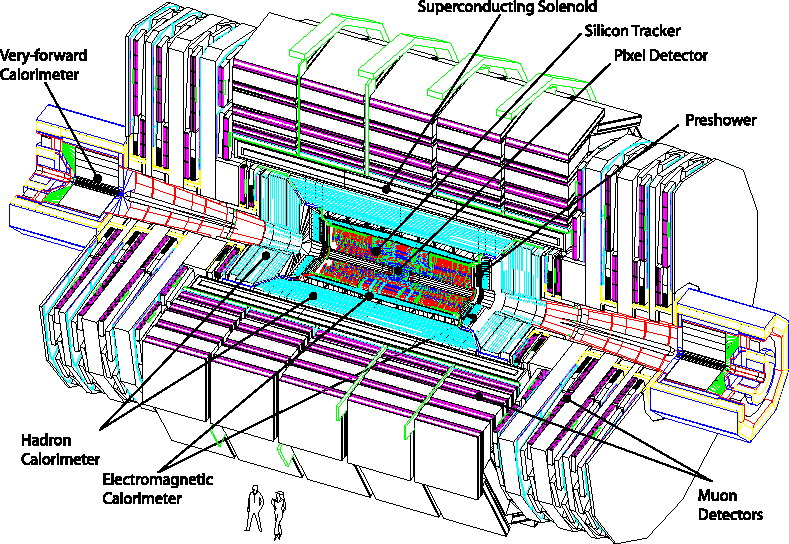
\includegraphics[width=.6\linewidth]{figures/CMS_view.pdf}
\caption{Основные элементы детектора CMS.}
\label{fig:view}
\end{figure*}

Качественная идентификация нейтральных пионов особенно важна, поскольку одной из мод распада бозона Хиггса является $H\to\gamma\gamma$, в которой образуются высокоэнергетичные фотоны. 
В свою очередь, нейтральный пион тоже распадается на два фотона, и если угол между ними достаточно мал, изначальная частица -- пион -- может быть неправильно определена как бозон Хиггса. 
Наибольшая вероятность такой ошибки возникает в близких к оси пучка областях. 

Близкая к пучку область, помимо уже описанной проблемы с пионами, выделяется еще многими уникальными для нее явлениями, поэтому конструкция детектора в ней несколько отличается от конструкции в цилиндрической части. 

\section{Основа калориметра}

Общий вид установки CMS представлен на Рис.~\ref{fig:view}. 
Электромагнитный калориметр целиком содержится внутри области, окруженной сверхпроводящим соленоидом, и покрывает область псевдобыстрот $|\eta|<3.0$. 
Все части калориметра сделаны из вольфрамата свинца, но перед близкими к пучку частями находится предлавинный детектор, служащий как раз для более точной идентификации нейтральных пионов. 
Сцинтилляционный свет регистрируется кремниевыми лавинными фотодиодами в параллельной пучку (цилиндрической) области и вакуумными фототриодами в перпендикулярной пучку области. 

Кристаллы вольфрамата свинца хорошо переносят радиацию, плотные и имеют маленькую радиационную длину, чуть меньше сантиметра, это позволило сделать компактный калориметр. 
Кроме того, их время испускания достаточно мало для использования на БАК: за 25 нс испускается порядка 80\% света. 

В цилиндрической части калориметра, содержащей 61 200 кристаллов, группы кристаллов помещаются в тонкостенные длинные подмодули, направленные к точке столкновения протонов. 
Группы подмодулей в зависимости от $\eta$ объединяются в модули, в каждом из которых оказывается по 400--500 кристаллов, покрывающих 20\degree{} по $\phi$. 
Четыре модуля объединяются в супермодуль. 
Такое объединение элементов детектора упрощает организацию считывающей электроники и охлаждения. 
В ближней к пучку части калориметра, содержащей по 7 300 кристаллов с каждой стороны, кристаллы объединяются в группы $5\times5$, называемые суперкристаллами. 
Кристаллы направлены в точку, находящуюся за 1.3 м за точкой столкновения протонов. 
Описанная конфигурация сцинтиллятора показана на Рис.~\ref{fig:crystals}.

\begin{figure}[b!]
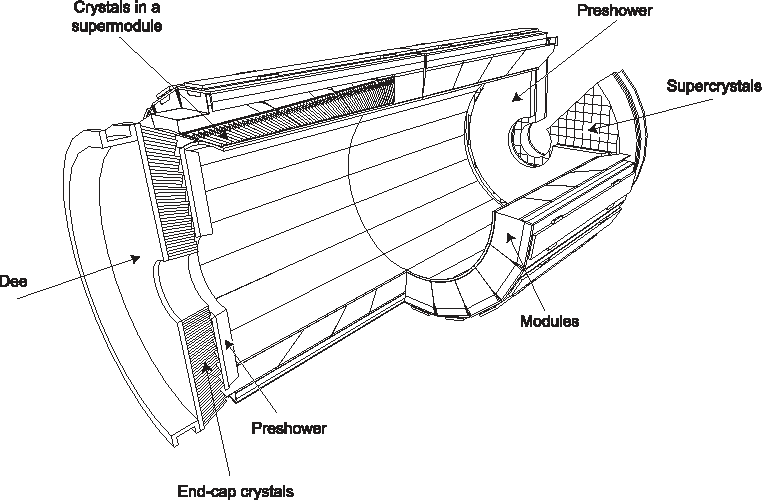
\includegraphics[width=.9\linewidth]{figures/Crystals}
\caption{Расположение и организация кристаллов в калориметре.}
\label{fig:crystals}
\end{figure}

Детекторы сцинтилляционных фотоном должны быть быстрыми, устойчивыми к радиации и способными работать в сильном магнитном поле. 
Кроме того, поскольку в сцинтилляторе образуется мало фотонов, необходимо усиливать сигнал. 
В сравнении с лавинными фотодиодами, вакуумные фототриоды, используемые в ближних к пучку участках калориметра, хоть и менее эффективны и слабее усиливают, но выдерживают значительно большую радиацию и способны работать даже в поле сверхпроводящего магнита CMS 4 Тл благодаря сверхтонким медным сеткам. 
Меньшая эффективность частично компенсируется лучшим покрытием поверхности на выходе сцинтиллятора. 

\section{Предлавинный детектор}
Предлавинный детектор занимает область псевдобыстрот  $1.65<|\eta|<2.6$ и нацелен в основном на идентификацию нейтральных пионов, рождающихся под малыми углами к протонному пучку.
Предлавинный детектор состоит из четырех слоев: в свинцовых радиаторах образуются электромагнитные ливни от падающих фотонов и электронов, а в кремниевых полосчатых сенсорах, расположенных за каждым из двух радиаторов, измеряются вклад энергии и поперечный профиль ливня.
Комбинации сенсора и считывающей электроники, называемые микромодулями, по 8 штук объединяются в лестницу. Лестницы образуют стандартную $x$-$y$ конфигурацию. 


\section{Электроника}
Считывающая электроника должна принимать маленькие сигналы фотодетекторов быстро и точно. 
Для качественной записи более широкого диапазона величин сигналов, предусилитель усиливает один и тот же сигнал параллельно в 1 раз, в 6 раз и в 12 раз, а затем выбирается самый наибольший сигнал, в котором еще не произошло насыщение. 
Для предотвращения влияния флуктуаций на выбор коэффициента усиления предусилитель переключается на более высокий коэффициент с задержкой.

В каждом событии на информацию из электромагнитного калориметра выделяется примерно 100~кБ, а для прочтения всей информации из калориметра потребовалось бы в 20 раз больше.
Естественно, не все части детектора интересны в каждом столкновении.
Для выделения и записи только важных его частей используется специальная система выборочного считывания.
Она учитывает вклады энергии, оставленные частицами в областях калориметра и вблизи них, и присваивает областям один из трех уровней интереса.
Наиболее интересные области и их соседи записываются целиком, области среднего интереса записываются целиком без соседей, а области малого интереса -- только если энергия в них превышает $3\sigma_\text{шум}$. 


\section{Наблюдение за калориметром}
Система контроля за калориметром отслеживает множество параметров детектора и окружающей среды и может уведомлять обслуживающий персонал о неполадках, а в случае угроз оборудованию детектора автоматически проводить необходимые процедуры. Система следит за температурой воздуха, влажностью, напряжением, охлаждением элементов детектора. 

Число испускаемых сцинтиллятором фотонов и усиление лавинными фотодиодами оба зависят от температуры, уменьшаясь при ее увеличении. 
Поэтому необходимо хорошо поддерживать температуру на постоянном уровне в пределах 0.05\degree{C}. 
Для стабилизации детектора система охлаждения использует воду, температура которой 18\degree{C}. 
Тесты показали, что построенная система охлаждения сохраняет температуру калориметра достаточно хорошо, чтобы температурные изменения в энергетическом разрешении были пренебрежимо малы. 

Также при наблюдении проводится калибровка детектора. 
В общих чертах калибровка калориметра представляет собой абсолютную энергетическую шкалу и относительную шкалу для сравнения данных между участками. 
Основной источник различий откликов областей калориметра в цилиндрической части -- изменения в сцинтилляционном свете от кристалла к кристаллу, имеющие дисперсию порядка 8\%. 
В ближних к пучку частях наибольший вклад дают вакуумные триоды, для них дисперсия составляет аж 25\%. 
Предварительное изучение используемой аппаратуры позволило уменьшить эти числа до 5\% и 10\% соответственно. 
Для дальнейшего улучшения этих показателей супермодули в собранном виде тестировались на космических лучах около недели, а затем 9 супермодулей -- на пучках высокоэнергетичных электронов. 
В результате относительная энергетическая погрешность внутри цилиндрической части калориметра составила 2\%. 
В ходе работы эксперимента CMS калибровка проводится на основе $p_T$ одиночных электронов (как в $W\to e\nu$) и масс $\pi_0$ и $\eta$ (распады на $\gamma\gamma$). 

Высокий уровень радиации и сильные потоки частиц приводят к образованию неоднородностей в веществе сцинтиллятора, а они, в свою очередь, частично поглощают волны некоторых длин. 
Такие повреждения приводят к установлению равновесия, зависящего от уровня радиации в текущий момент. 
Этот процесс можно отслеживать и учитывать с помощью лазерной системы наблюдения за оптической прозрачностью. 
Прозрачность вещества устанавливается, исходя из отношения зарегистрированного фотодетекторами света к импульсу лазера, причем необходимо учесть, что оптический путь в сцинтилляторе меняется и спектр лазера не идеально совпадает со спектром сцинтиллятора. 
С учетом этого прозрачность вещества зависит от названного отношения степенным законом. 

\section{Энергетическое разрешение}
Для энергий меньше 500 ГэВ, при которых утечка частей ливня в калориметре становится значительной, энергетическое разрешение $\sigma$ можно разделить на три компоненты: стохастическую, шумовую и постоянную
$$ \left( \sigma \over E \right)^2 = \left( S \over \sqrt{E} \right)^2 + \left( N \over E \right)^2 + C^2. $$

В стохастическую компоненту входят флуктуации от события к событию, статистические флуктуации из-за числа фотонов и флуктуации во вкладе энергии, оставленном в предлавинной системе, с учетом измеренного предлавинными силиконовыми детекторами. 
Наибольшие вклады в постоянную компоненту дают неоднородное в продольном направлении поглощение кристаллами света, ошибки в относительной калибровке и утечка энергии с задней поверхности кристалла (для поздно начавшихся ливней). 
Продольная неоднородность кристаллов частично компенсирует утечку энергии с задней поверхности. 
В шумовой компоненте тоже три вклада: шум электроники, шум, возникающий при оцифровке данных, и шум от множественных взаимодействий в протонных пучках. 
Шумы электроники и оцифровки снижаются за счет того, что амплитуда в каждом канале вычисляется с учетом постоянного значения, которое выдавал этот канал в три предшествовавших импульсу момента времени. 
Успех этой процедуры подтверждается зависимостью $\sigma_N^\text{шум} \approx \sqrt{N}\,\sigma_1^\text{шум}$ при считывании с $N$ каналов. 

Полученные в предварительном (до работы на БАК) исследовании значения оказались следующими (для $E$ в ГэВ): 
$$ \left( \sigma \over E \right)^2 = \left( 0.028 \over \sqrt{E} \right)^2 + \left( 0.12 \over E \right)^2 + 0.0030^2. $$
Постоянный член довольно мал, поэтому разрешение ухудшается практически линейно с энергией, как видно на Рис.~\ref{fig:graph}.









\nocite{CMS_JINST}
%%%%%%%%%%%%%%%%%%
%% Bibliography %%
%%%%%%%%%%%%%%%%%%
\bibliographystyle{local}
\bibliography{Refs}

\newpage
\null
\begin{figure}
\begin{tikzpicture}
\begin{axis}[
	xlabel={$E$ (ГэВ)},
	ylabel={$\sigma$ (ГэВ)},
	xmin=.5, xmax=1000,
	xmode=log, 
	ymode=log,
]
	\addplot[domain=0.5:1000, black]{sqrt(0.12*0.12+0.028*0.028*x+0.003*0.003*x*x)};
\end{axis}
\end{tikzpicture}
\caption{Разрешение электромагнитного калориметра CMS.}
\label{fig:graph}
\end{figure}

\end{document}





\begin{thebibliography}{9}
\bibitem{CMS_JINST} S. Chatrchyan \textit{et al}. (CMS Collaboration), The CMS experiment at the CERN LHC, \href{dx.doi.org/http://dx.doi.org/10.1088/1748-0221/3/08/s08004}{JINST \textbf{3}, S08004 (2008)}.
\end{thebibliography}
